\documentclass{article}
\usepackage{graphicx}
\usepackage[framed, numbered]{matlab-prettifier}
\usepackage[margin = 0.8 in]{geometry}
\usepackage{amsmath}
\usepackage{placeins}
\usepackage{listings}
\usepackage{xcolor}
\usepackage{cite} 
\usepackage{url}
\usepackage{indentfirst}

\usepackage[utf8]{inputenc}
\usepackage[english]{babel}

\setlength{\parindent}{3em}
\setlength{\parskip}{0em}

\definecolor{codegreen}{rgb}{0,0.6,0}
\definecolor{codegray}{rgb}{0.5,0.5,0.5}
\definecolor{codepurple}{rgb}{0.58,0,0.82}
\definecolor{backcolour}{rgb}{0.95,0.95,0.92}

\lstdefinestyle{mystyle}{
    backgroundcolor=\color{backcolour},   
    commentstyle=\color{codegreen},
    keywordstyle=\color{magenta},
    numberstyle=\tiny\color{codegray},
    stringstyle=\color{codepurple},
    basicstyle=\ttfamily\footnotesize,
    breakatwhitespace=false,         
    breaklines=true,                 
    captionpos=b,                    
    keepspaces=true,                 
    numbers=left,                    
    numbersep=5pt,                  
    showspaces=false,                
    showstringspaces=false,
    showtabs=false,                  
    tabsize=2
}

\begin{document}

\title{Assembly line of MatLab, Matplotlib, and \LaTeX{}}
\author{Shreedhar Jangam}

\maketitle

\section{Introduction}
	Objective of this project is to learn the uses and analyze the relationship between MatLab \cite{matlabtool}, Matplotlib \cite{matplotlibtool}, and LaTex \cite{latextool}. Matlab was used to produce data points. Matplotlib was used to produce a graph. Finally, Latex was used to write the report.\par 
	As a beginner, I used various online tutorials, websites and videos to learn the applications of these softwares. Quick online searches about the errors or new features progressively built my knowledge.\par
	Knowledge of these software can be beneficial while writing project reports, research papers, and presentations. You start by programming a mathematical model/simulation in MatLab, generate the visualizations using the data generated by the model using Matplotlib, and prepare the report of  your findings using LaTex. All these skills will make your research paper look fantastic.

\section{MatLab}
\subsection{MatLab Code}
MatLab is given an equation which it graphs and extracts coordinates within given the range. Next, it compiles the code and produces a Excel and a PNG file. The Excel file contains a table with x and y values and the PNG file contains the graph. Code is written in MatLab and embedded in LaTex\cite{matlabvid}. 

\lstinputlisting[style=Matlab-editor, caption={Quadratic Equation Model in MatLab}]{getting_cordinates_from_graph.m}

\subsection{MatLab Plot}
MatLab graphed the equation \(y = x^2\) in the range $-10 \leq x \geq 10$. The plot was saved as a png file \cite{matlabcode}. Check out the plot~\ref{fig:matlabfigure} on page \pageref{fig:matlabfigure}. 
\begin{figure}[h]
    \centering
   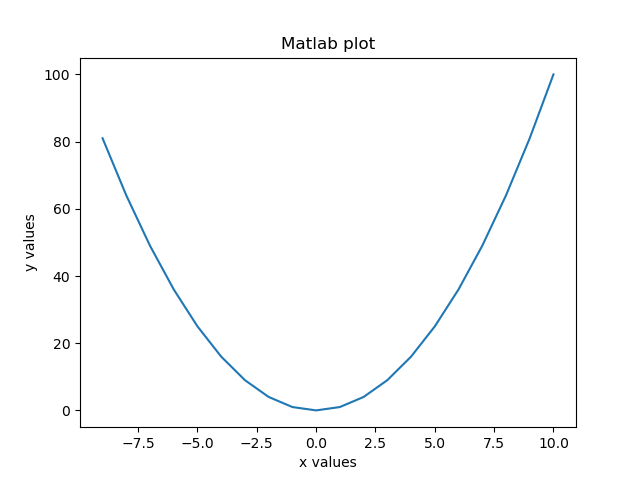
\includegraphics[scale=1]{../../MatLab/quad_coordinates.png} 
    \caption{MatLab Simulation Results}
    \label{fig:matlabfigure}
\end{figure}

\section{Matplotlib}
You can learn more about the Matplotlib library by auditing a coursera couse on Matplotlib called "Applied Plotting, Charting \& Data Representation in Python" \cite{matplotlibcoursera}

\subsection{Matplotlib Code}
Matplotlib imports the Excel file produced by MatLab and plots the coordinates. Matplotlib code is written in Python and embedded in LaTex\cite{matplotlibcode}. 

\begin{lstlisting}[language=Python, style=mystyle]
// coordinates.py
import xlrd
import os
import matplotlib.pyplot as plt
from matplotlib.backends.backend_agg import FigureCanvasAgg

# setting up the canvas
fig = plt.figure()
canvas = FigureCanvasAgg(fig)

# accessing the xlsx file
cwd = os.getcwd()
data_file = 'c:\workspace\shree\MatLab\quad_coordinates.xlsx'
book = xlrd.open_workbook(data_file)
sheet = book.sheet_by_name("Sheet1")

# reading coordinates from the xlsx file
col_x_vals = sheet.col_values(0, 2)
col_y_vals = sheet.col_values(1, 2)

# plotting the coordinates
plt.plot(col_x_vals, col_y_vals)

# customizing the figure
plt.xlabel('x values')
plt.ylabel('y values')
plt.title('Matplotlib plot')

# saving the figure
canvas.print_figure('images/quad_coordinates.eps')
canvas.print_figure('c:\workspace\shree\LaTex\project_report\images\quad_coordinates.eps')

\end{lstlisting}

\subsection{Matplotlib Plot}
Matplotlib was used to plot the results and out plot was compared with the one produced by MatLab. The Excel file was imported in Matplotlib and read to get the output data values generated by the model. These values then plotted using the plot function. 

After comparing both plots, it was found that the results were similar. Check out the plot~\ref{fig:matplotlibfigure} on page \pageref{fig:matplotlibfigure}.

\begin{figure}[h]
    \centering
        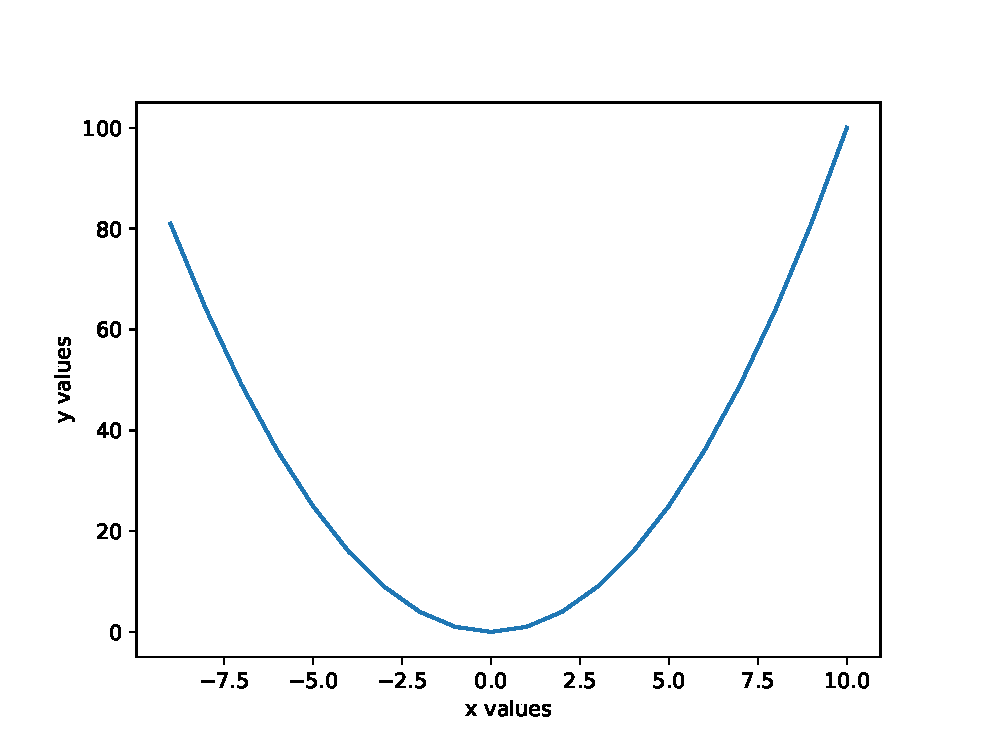
\includegraphics[scale = 1]{../../pyprogs/pyvisual/pyvis/images/quad_coordinates.eps} 
    \caption{Matplotlib Simulation Results}
    \label{fig:matplotlibfigure}
\end{figure}

\section{LaTex}
LaTex imports both - the code written for MatLab and Matplotlib and the generated plots. All four elements are used to create this report.

\section{Conclusion}
Both the plots created by MatLab and Matplotlib are similar and follows the quadratic curve. Therefore, it can be concluded that the code is working. 

\bibliography{quadmodelbib} 
\bibliographystyle{ieeetr}

\end{document}